\documentclass[twocolumns]{udes_rapport}
% Si on préfère avec une seule colonne :
% \documentclass[onecolumn]{udes_rapport}

% pour les tableaux
\usepackage{tabularray}
\UseTblrLibrary{booktabs}
\usepackage[table]{xcolor}
\usepackage{adjustbox}

% pour la bibliographie
\usepackage[backend=biber]{biblatex}
\usepackage{csquotes}
\addbibresource{Source/bibliography.bib}


\begin{document}

\title{
    Classement des universités mondiales de 2017 à 2022 par Quacquarelli Symonds
}
\author{
    Ala Antabli\and Josselin Dubois\and Antoine Guénard\and Gurleen Padda\footnote{anta2801, dubj0701, guea0702, padg5000}
}

\maketitle

\section{Introduction}\label{sec:introduction}

    \subsection{À propos du classement}\label{subsec:ranking}

        QS World University Rankings est une publication annuelle des classements mondiaux des universités par Quacquarelli Symonds. Ce classement est considéré comme l'un des trois classements universitaires les plus pertinents au monde. Il reçoit également l'approbation du groupe d'experts sur le classement international (IREG). QS publie ses classements universitaires en partenariat avec Elsevier.

    \subsection{L'importance du sujet}\label{subsec:subject_importance}
    
        Dans les premières années de nos vies notre établissement scolaire est le plus proche de chez nous. Arrivé à l'université, on est nombreux à vouloir faire le choix de l'excellence pour nos études. Les classements ont cette vocation. Mais ces classements peuvent également être révélateurs d'inégalités dans l'accès aux études, que ce soit pour les étudiants dans des zones défavorisés, ou même pour les étudiants internationaux. Il est ainsi intéressant, voire primordial, de se renseigner sur les différents facteurs qui rendent une université mieux classée qu'une autre. Cela peut aussi être un indicateur pour les universités elles-même pour savoir sur quoi se concentrer dans l'objectif d'améliorer son attractivité.
        
        Étant en plein dans les études universitaires, on a tous déjà regardé ces fameux classements, notamment pour s'intéresser aux universités étrangères. C'est donc naturellement que nous nous intéressons à cette base de donnée.
        De plus, nous sommes tous les 4 étudiants d'horizons différents, et donc tous touchés par les enjeux de tels classements.

\section{Contexte scientifique}\label{sec:context}

    Sur notre jeu de données, seuls deux travaux de visualisation ont été effectués, par Padhma Muniraj \cite{trav1} et Naiva Piatchou \cite{trav2}, décrivant quelques liens entre les variables du jeu de données, après avoir nettoyé les données.

    Cependant, de vrais travaux d'analyse n'ont été efféctués que sur d'autres jeux de données, similaires, mais avec des variables différentes, dans le but de retrouver le score et le classement des universités à partir des variables. Parmi ces travaux, on peut mentionner ceux de Shubham Kamble \cite{trav3} qui, en utilisant des méthodes de régression (régression linéaire, puis RandomForest, et enfin XGBoost), avait prédit avec une bonne précision les scores et le classement des universités. On peut aussi mentionner les travaux de Jeremy Leipzig \cite{trav4}, plus anciens : ce dernier avait effectué une analyse en composantes principales, en conservant les 3 premières composantes principales qui expliquaient respectivement 42\%, 11\% et 8\% de la variance totale. D'autres travaux, plus rares, avaient effectué du clustering, mais étaient orientés sur la comparaison du classement QS avec d'autres systèmes de notation : on les laissera donc de côté.

\section{Travail proposé}\label{sec:work}

    Notre projet vise à développer un outil de prédiction des niveaux des universités et essayer de comprendre ce qui fait d'une université une bonne université.
    
    Nous allons donc faire une classification sur toutes les données pour classifier les universités dans 11 groupes, où les universités du groupe $i$ sont « meilleures » que celles du groupe $i+1$. Le groupe $1$ devrait être constitué des « meilleures » universités, et et le groupe 11 devrait être constitué des « moins bonnes » universités. En parallèle, on essaiera de faire des régressions sur le score des universités.


\section{Description des données}\label{sec:data_description}


    Les données sont constituées de $13$ attributs, ainsi que le score et les classements des universités pour les années de 2017 à 2022. Il y a $1368$ universités nommées dans ces données, mais toutes les universités n’apparaissent pas à chaque année, donc il y a au total $6482$ objets. Les attributs sont :
    
    \begin{enumerate}
        \item \textbf{university} : Le nom de l’université (\emph{string}).
        \item \textbf{year} : L’année du classement (\emph{int}). 
        \item \textbf{rank\_display} : Le classement (\emph{int}). Le classement est attitré en ordre croissant, c’est-à-dire que l’université avec classement $1$ est la « meilleure » et celle avec le plus grand classement est la « pire ».
        \item \textbf{score} : Le score (sur 100\%) que QS a calculé pour l’université qui détermine le classement (\emph{float}). Le score est basé sur \cite{score}:
        \begin{itemize}
            \item (40\%) La réputation académique selon un sondage de plus de $130 000$ individus qui travaillent aux études supérieures
            \item (10\%) La réputation selon les employeurs, où on demande aux employeurs d’identifier les universités d’où ils obtiennent les meilleurs employés.
            \item (20\%) Le proportion de faculté par étudiant
            \item (20\%) Le nombre de citations par faculté dans les 5 dernières années. Les données sont normalisées puisque dans certaines facultés il y a plus ou moins de publications en général.
            \item (5\%) Le proportion de membres de faculté international
            \item (5\%) Le proportion d’étudiants internationaux
        \end{itemize}
        \item \textbf{link} : Un lien vers le profil de l’université sur le site web de QS.
        \item  \textbf{country} :Le pays où l’université se situe (\emph{categorical}).
        \item \textbf{city} : La ville où l’université se situe (\emph{categorical}).
        \item \textbf{region} : Le continent sur lequel l’université se situe (\emph{categorical}).
        \item \textbf{logo} : Un lien qui mène vers le logo de l’université.
        \item \textbf{type} : Le type (privé ou public) de l'université (\emph{categorical}).
        
        \item \textbf{research\_output} : Une classification de la qualité des résultats de recherche (\emph{categorical}).
        
        \item \textbf{student\_faculty\_ratio} : Le proportion de faculté par étudiant (\emph{float})
        
        \item \textbf{international\_students} : Le nombre d’étudiant internationnaux (\emph{int}).
        
        \item \textbf{size} : La superficie des campus (\emph{categorical}).
        
        \item \textbf{faculty\_count} : Le nombre de membres de facultés et du personnel académique (\emph{int}).
    \end{enumerate}

    On peut voir dans la figure \ref{fig:mis_vals} qu'il y a des valeurs manquants dans les données. Pour les universités qui sont classées plus haut que $500$ il n'y a pas de score disponible, donc pour à peu près la moitié des données il n'y a pas de score. D'autres attributs disposent légèrement de valeurs manquantes. Le problème sera réglé dans 
    Il y a aussi d'autres attributs qui manquent des valeurs et nous allons les adresser lors du nettoyage des données.
    
    \begin{figure}[h!]
        \centering
        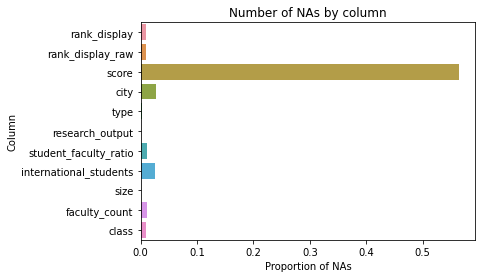
\includegraphics[scale=0.5]{Images/na_proportion_2.png}
        \caption{Proportion de valeurs manquantes par attributs (seulement celles avec au moins une valeur manquante)}
        \label{fig:mis_vals}
    \end{figure}


\section{Analyse brute des données}\label{sec:raw_analysis}

    On a commencé par observer manuellement la distribution de notre jeu de données. En particulier, on s'intéresse à la corrélation entre nos différents attributs. On dresse pour cela la matrice de corrélation (voir la figure \ref{fig:corr_matrix}). Celle-ci nous permet de constater que nos attributs semblent très indépendants. Seuls le nombre d'étudiants internationaux semble légèrement lié au nombre de personnels et de facultés, ce qui semble logique.
    
    En dressant ensuite le graphique des 3 attributs les plus liés entre eux selon la matrice (\emph{student\_faculty\_ratio}, \emph{international\_students} et \emph{faculty\_count}, voir figure \ref{fig:pairgrid}), on remarque effectivement une légère tendance à aller dans le même sens, sans pour autant pouvoir en distinguer une corrélation linéaire.
    
    \begin{figure}[h!]
        \centering
        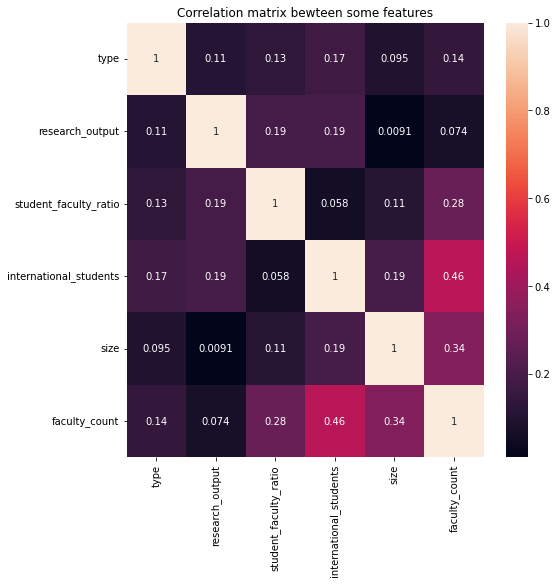
\includegraphics[scale=0.45]{Images/corr_matrix.png}
        \caption{Matrice de corrélation entre certains attributs}
        \label{fig:corr_matrix}
    \end{figure}
    

    \begin{figure}[h!]
        \centering
        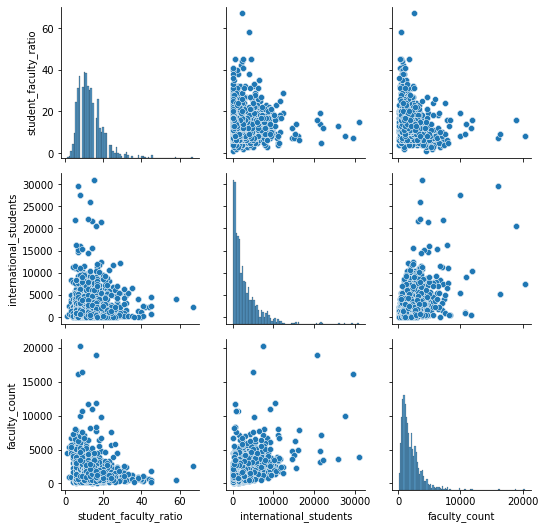
\includegraphics[scale=0.4]{Images/pairgrid.png}
        \caption{Visualisation des attributs en fonction des autres}
        \label{fig:pairgrid}
    \end{figure}
    
    Finalement, il nous semblait intéressant d'observer la distribution de certains attributs en fonction de la classe (donc du classement) de l'université. Cela permettrait d'avoir une première intuition des critères importants qui font qu'une université est bien classée ou non. On visualise ainsi la qualité du niveau de recherche (figure \ref{fig:research_output_by_class}), le nombre de facultés par étudiants (figure \ref{fig:student_faculty_ratio_by_class}), le nombre d'étudiants internationaux (figure \ref{fig:international_students_by_class}) ainsi que le nombre de personnels (figure \ref{fig:faculty_count_by_class}).
    
    Sur la figure \ref{fig:research_output_by_class} (concernant le niveau de recherche), il est fragrant de voir que mieux l'université est classée, plus l'université a un bon niveau de recherche. Ainsi, le nombre d'universités avec un niveau de recherche très élevé (en bleu) diminue lorsque le classement baisse, tandis que le nombre d'université avec un niveau de recherche élevé (en orange) ou moyen (en vert) augmente.
    
    Sur les 3 autres figures, on remarque également que la moyenne est toujours une fonction monotone en fonction de la classe. Ainsi, un ratio élevé entre le nombre de facultés par étudiant implique d'être moins bien classé. À contrario, un meilleur nombre d'étudiants internationaux ou de membres de personnel implique d'être mieux classé.
    
    \begin{figure}[h!]
        \centering
        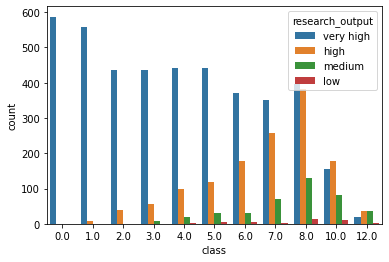
\includegraphics[scale=0.6]{Images/research_output_by_class.png}
        \caption{Nombre d'universités avec un certain niveau de recherche en fonction de la classe}
        \label{fig:research_output_by_class}
    \end{figure}
    
    \begin{figure}[h!]
        \centering
        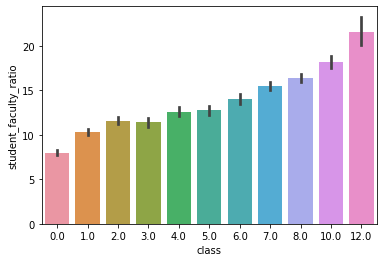
\includegraphics[scale=0.6]{Images/student_faculty_ratio_by_class.png}
        \caption{Moyenne et écart-type du nombre de facultés par étudiants en fonction de la classe}
        \label{fig:student_faculty_ratio_by_class}
    \end{figure}
    
    \begin{figure}[h!]
        \centering
        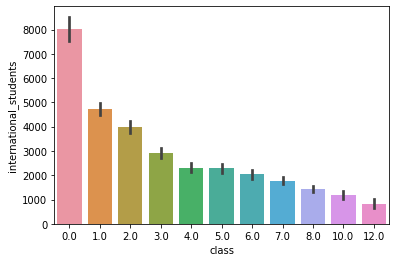
\includegraphics[scale=0.6]{Images/international_students_by_class.png}
        \caption{Moyenne et écart-type du nombre d'étudiants internationaux en fonction de la classe}
        \label{fig:international_students_by_class}
    \end{figure}
    
    \begin{figure}[h!]
        \centering
        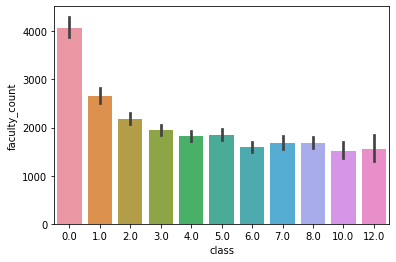
\includegraphics[scale=0.6]{Images/faculty_count_by_class.png}
        \caption{Moyenne et écart-type du nombre de personnels en fonction de la classe}
        \label{fig:faculty_count_by_class}
    \end{figure}
    
    On visualise enfin les régions des universités selon leurs tranche de classement (figure \ref{fig:region_by_class}), mais celles-ci semblent plus ou moins uniformément réparties entre les différents classements.
    
    \begin{figure}[h!]
        \centering
        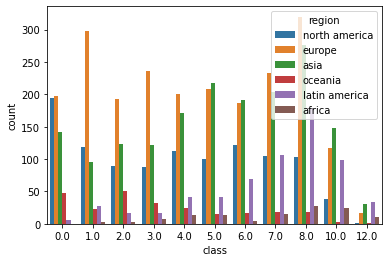
\includegraphics[scale=0.6]{Images/region_by_class.png}
        \caption{Nombre d'universités d'une certaines région en fonction de la classe}
        \label{fig:region_by_class}
    \end{figure}

\section{Nettoyage des données}\label{sec:cleaning}
    
    \subsection{Analyse et modifications}\label{subsec:analyis_modifications}
        
        En analysant la base de données, on a détecté plusieurs colonnes inutiles à l'analyse.

        Les colonnes \textsf{link} et \textsf{logo} (contenant respectivement un lien vers le site de l'université et l'image du logo) ont ainsi été supprimées.
        
        Les colonnes \textsf{university} et \textsf{year} ne contiennent que des informations pour identifier les lignes. On les a donc regroupées en une unique colonne \textsf{university\_with\_year}.
        
        Les rangs des universités étaient parfois données par tranche (500-600 par exemple), alors qu'on aimerait des entiers. On modifie alors toutes les tranches par la valeur minimale (500-600 devient 500).
        
        Finalement, on a ajouté la colonne \textsf{classe} pour le bien de la classification. Ainsi, on a divisé les universités en 12 classes, où a $i$-ème classe contient les universités classées de $100i$ à $100(i+1) - 1$ (la classe 0 contient ainsi les universités classées de 0 à 99). La figure \ref{fig:classe_distrib} en montre la distribution.
        
        \begin{figure}[h!]
            \centering
            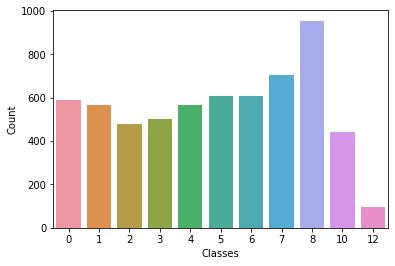
\includegraphics[scale=0.5]{Images/classe_distribution.png}
            \caption{Distribution de la colonne \textsf{classe}}
            \label{fig:classe_distrib}
        \end{figure}
    
    \subsection{Données manquantes}\label{subsec:missing_values}
    
        La base de données contenait un certain nombre de données manquantes (4115 cellules, soit 4\% des celulles ; réparties sur 3703 lignes, soit 57\% des lignes) On montre la réparition de ces données manquantes sur la figure \ref{fig:na_prop}. Fort heureusement, nous étions capable de remplir bon nombre de ces valeurs manquantes.
    
        \begin{figure}[h!]
            \centering
            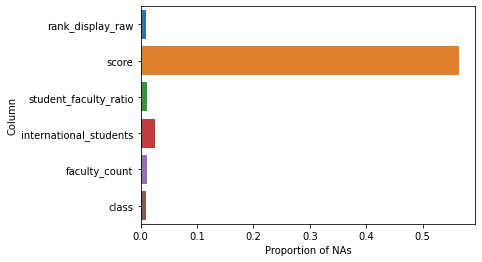
\includegraphics[scale=0.5]{Images/na_proportion.png}
            \caption{Distribution de la colonne \textsf{classe}}
            \label{fig:na_prop}
        \end{figure}
        
        D'abord, on peut remplir le score pour certaines données manquantes. En effet, certaines universités sans score avaient le même rang que certaines université avec score. On a alors pu copier les scores de ces dernières pour remplir les premières. On rempli ainsi 183 données, soit 3\% des données.
        
        De part leur nature, on a également pu remplir les colonnes \textsf{student\_faculty\_ratio}, \textsf{international\_students} et \textsf{faculty\_count} avec la médiane des colonnes. Cela remplit 211 données, soit 3\% des données.
        
        Finalement, on supprime toutes les lignes ayant au moins 2 colonnes nulles. Cela supprime 68 lignes, soit 2\% des données. On peut de plus noter que seule la colonne \textsf{score} ne comporte finalement des données nulles.
        
        On a ainsi supprimé 640 valeurs nulles, soit 15\% des données nulles.

    \subsection{Données aberrantes}\label{subsec:outliers}
    
        En parcourant la base de données, on a constaté quelques données aberrantes, c'est à dire avec un rang qui ne correspond pas à leur score. On a ainsi supprimé les universités $i$ et $j$ telles que score($i$) $>$ score($j$) mais rang($i$) $>$ rang($j$).

        On supprime ainsi 305 données, soit 5\% des données.
    
\section{Algorithmes utilisés}\label{sec:algorithms}

    Dans les algorithmes suivants, on n'essaiera pas de retrouver les rangs précis des universités, mais plutôt de retrouver la classe (créée artificiellement), ce qui est largement suffisant.

    \subsection{Régression linéaire}\label{subsec:lm}
    
        On commence par tester un modèle linéaire simple pour effectuer une régression sur la classe de nos universités. On prend ensuite la classe la plus proche du résultat obtenu pour effectuer une classification. On utilise pour cela la classe \href{https://scikit-learn.org/stable/modules/generated/sklearn.linear_model.LinearRegression.html}{\textsf{LinearRegression}} de la bibliothèque \textsf{scikit-learn}. 

    \subsection{Arbre de décision}\label{subsec:tree}
    
        On décide ensuite de tester un arbre de décision pour classifier selon la classe, qui permet de classifier un ensemble de données en suivant un ensemble de décisions simples organisées sous forme d'arbre. On utilise pour cela le classifieur \href{https://scikit-learn.org/stable/modules/generated/sklearn.tree.DecisionTreeClassifier.html}{\textsf{DecisionTreeClassifier}} de la bibliothèque \textsf{scikit-learn}. Pour donner une idée de la forme et la complexité d'un tel arbre, on montre sur la figure \ref{fig:tree} l'arbre obtenu.
        
        \begin{figure}[h!]
            \centering
            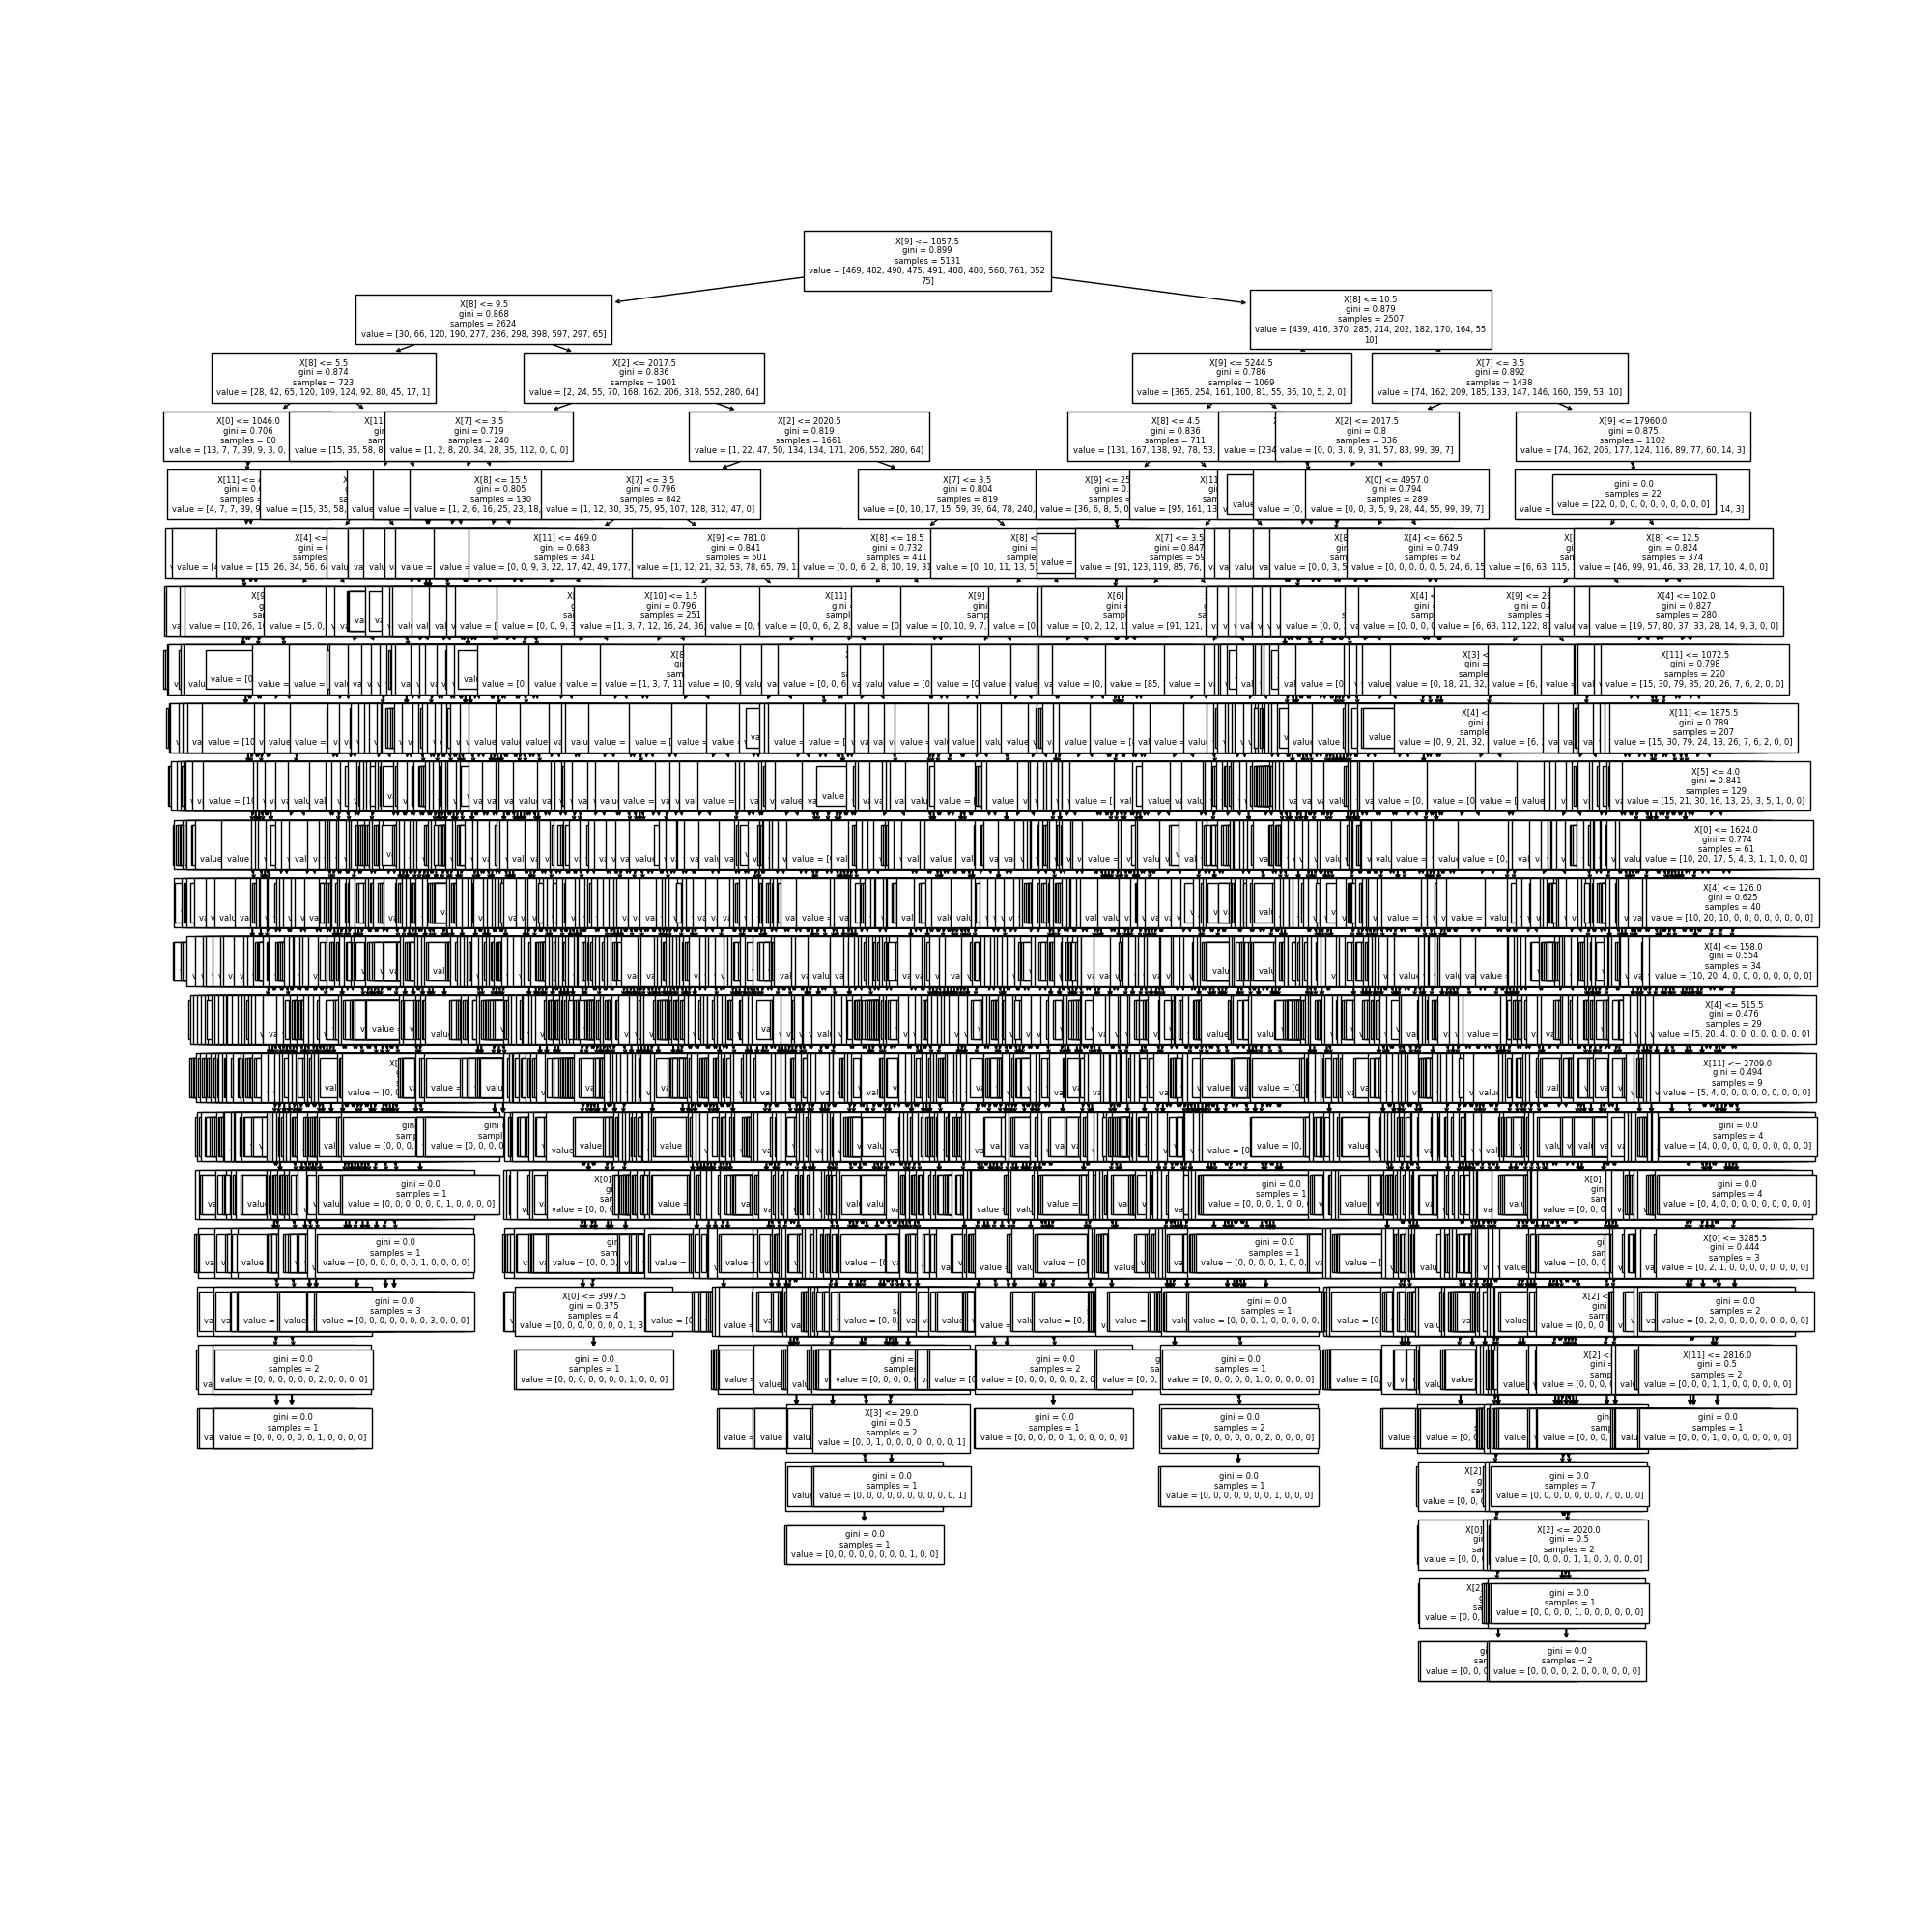
\includegraphics[width=7cm, height=5cm]{Images/tree_results.png}
            \caption{Visualisation de l'arbre résultant}
            \label{fig:tree}
        \end{figure}

    \subsection{XGBoost}\label{subsec:xgboost}
    
        Suite logique à l'arbre de décision, on utilise ensuite la méthode \href{https://xgboost.readthedocs.io/en/stable/python/python_api.html#module-xgboost.sklearn}{\textsf{XGBoost}}, qui est une combinaison d'arbres de décision. On l'utilise à deux escients : d'abord pour effectuer une régression sur le score (à l'aide de la classe \textsf{XGBRegressor}), ensuite pour effectuer une classification sur la classe (à l'aide de la classe \textsf{XGBClassifier}).
    
\section{Métriques utilisées}\label{sec:metrics}

    Différentes métriques ont été utilisées pour mesurer la performance de nos prédictions.
    
    \subsection{Classification}\label{subsec:metrics_clf}
    
        Pour la classification, on utilise les 4 métriques suivantes :
        \begin{itemize}
            \item \href{https://scikit-learn.org/stable/modules/generated/sklearn.metrics.accuracy_score.html}{Exactitude} : proportion de données bien classées
            
            \item \href{https://scikit-learn.org/stable/modules/generated/sklearn.metrics.precision_score.html}{Précision} : moyenne des ratios \textsf{tp / (tp + fp)} (abilité à bien classé négatif une donnée négative) pour chaque classe
            
            \item \href{https://scikit-learn.org/stable/modules/generated/sklearn.metrics.recall_score.html}{Rappel} : moyenne des ratios \textsf{tp / (tp + fn)} (abilité à trouver les données positives) pour chaque classe
            
            \item \href{https://scikit-learn.org/stable/modules/generated/sklearn.metrics.jaccard_score.html}{Jaccard} : Moyenne des ratios \textsf{intersection / union} (similarité) pour chaque classe
        \end{itemize}
    
    \subsection{Regression}\label{subsec:metrics_reg}
    
        Pour la régression, on utilise les 3 critères suivants :
        \begin{itemize}
            \item \href{https://scikit-learn.org/stable/modules/generated/sklearn.metrics.explained_variance_score.html}{Variance expliquée} : proportion de la variance expliquée par la régression
            
            \item \href{https://scikit-learn.org/stable/modules/generated/sklearn.metrics.mean_squared_error.html}{RMSE} : racine de la moyenne des erreurs au carré
            
            \item \href{https://scikit-learn.org/stable/modules/generated/sklearn.metrics.r2_score.html}{R$^2$} : coefficient de détermination linéaire
        \end{itemize}

    
\section{Analyse des résultats}\label{sec:results}

    \subsection{Scores des modèles}\label{subsec:scores}
    
        Les scores ont été obtenus en prenant la moyenne des résultats obtenus pour divers jeux de validation.
        
        \begin{itemize}
            \item Pour la classification :
            
            La figure \ref{tbl:scores_clf} montre les scores obtenus pour nos modèles de classification sur la classe. 
            \begin{table}
                \centering
                \scalebox{0.85}{
                \begin{tblr}{
                    colspec={l *4c},
                    row{1}={font=\mdseries},
                    column{1}={font=\mdseries},
                    row{even}={bg=gray!10},
                }
                \toprule
                    Algorithme & Exactitude & Précision & Rappel & Jaccard  \\\midrule
                    Modèle linéaire & 0.18 & 0.18 & 0.18 & 0.10 \\
                    Arbre de décision & 0.61 & 0.57 & 0.57 & 0.43 \\ 
                    XGBoost & 0.65 & 0.65 & 0.65 & 0.48\\\bottomrule
                \end{tblr}
                }
                \caption{Scores des modèles de classification}
                \label{tbl:scores_clf}
            \end{table}
    
            Le modèle linéaire produit des résultats très faibles, ce modèle est loin d'être fiable pour notre étude de cas. L'arbre de décision améliore grandement le modèle, même si les résultats ne sont toujours pas parfaits. Ce dernier est encore légèrement amélioré par la méthode \textsf{XGBoost}, qui obtient des résultats légèrement satisfaisants.

            \item Pour la régression :
            La figure \ref{tbl:scores_reg} montre les scores obtenus pour nos modèles de régression sur le score. 

            \begin{table}
                \centering
                \begin{tblr}{
                    colspec={l *3c},
                    row{1}={font=\mdseries},
                    column{1}={font=\mdseries},
                    row{even}={bg=gray!10},
                }
                \toprule
                    Algorithme & Variance expliquée & RMSE & R$^2$ \\\hline
                     Modèle linéaire & 0.54 & 4.31 & 0.54 \\
                     XGBoost & 0.90 & 34.96 & 0.90\\\bottomrule
                \end{tblr}
                \caption{Scores des modèles de régression}
                \label{tbl:scores_reg}
            \end{table}
                
            Encore une fois, le modèle linéaire n'est pas satisfaisant, même s'il est meilleur que pour la classification. En revanche, la méthode \textsf{XGBoost} obtient des excellent résultats (variance expliquée et $R^2$ très proches de 1).
            
        \end{itemize}
    
    \subsection{Interprétation}\label{subsec:interpretation}
    
        Les deux méthodes XGBoost produisent des résultats satisfaisants, on peut donc s'intéresser de plus près à ce qu'ils nous disent.
    
        \begin{figure}[h!]
            \centering
            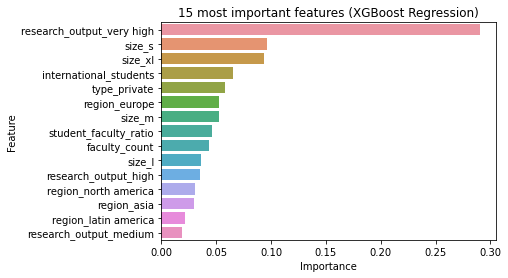
\includegraphics[scale=0.5]{Images/important_features_xgbreg.png}
            \caption{15 attributs les plus importants selon XGBoost (Régression)}
            \label{fig:imp_features_xgbreg}
        \end{figure}
        \begin{figure}[h!]
            \centering
            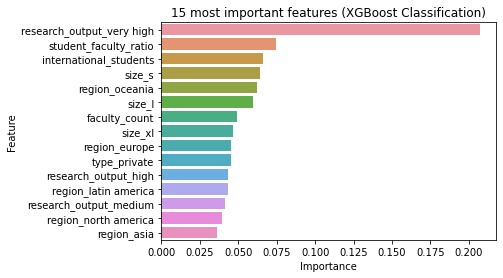
\includegraphics[scale=0.5]{Images/important_features_xgbclf.png}
            \caption{15 attributs les plus importants selon XGBoost (Classification)}
            \label{fig:imp_features_xgbclf}
        \end{figure}

        Une évidence se dégage de ces deux résultats : l'importance du niveau de recherche de l'établissement est primordial (\textsf{very high} est largement premier dans les deux classements, et on note la présence des niveaux \textsf{high} et \textsf{medium}). On note également que la présence d'étudiants internationaux (\textsf{international\_students}) joue dans les deux cas (sûrement lié au fait que les meilleures universités attirent les étudiants internationaux). La region semble également assez présente (on voit notamment l'europe, l'asie et l'amérique du nord). Finalement, on note la présence de la taille de l'université, ainsi que le fait que l'université soit privée ou non.
        
        Bien qu'ayant des résultats moindres, on peut aussi s'intéresser aux variables importantes du modèle linéaire et de l'arbre de décision :
        
        \begin{figure}[h!]
            \centering
            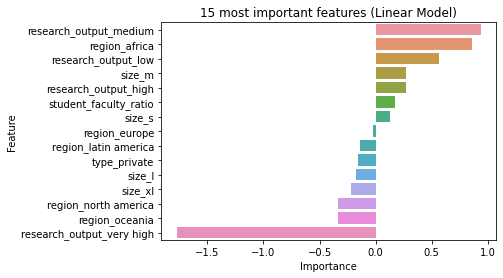
\includegraphics[scale=0.5]{Images/important_features_lm.png}
            \caption{15 attributs les plus importants selon l'arbre de décision}
            \label{fig:imp_features_xgbreg}
        \end{figure}
        
        \begin{figure}[h!]
            \centering
            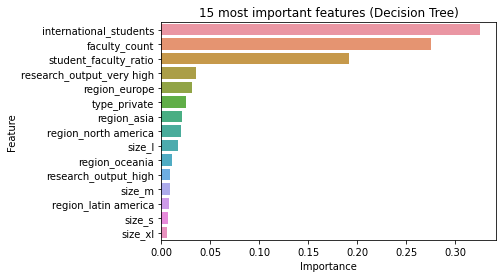
\includegraphics[scale=0.5]{Images/important_features_tree.png}
            \caption{15 attributs les plus importants selon le modèle linéaire}
            \label{fig:imp_features_xgbclf}
        \end{figure}
        
        Pour le modèle linéaire, on retrouve comme pour les autres modèles l'importance du niveau de recherche très élevé, les régions Amérique du Nord et Europe, le caractère privé ainsi que la taille élevée pour obtenir une classe faible (donc un meilleur classement). À l'inverse, un niveau de recherche moindre ou un gros ratio mène à une classe plus élevée (donc à un moins bon classement).
        
        Les résultats de l'arbre de décision sont similaires aux 3 autres modèles, bien que celui-ci met une plus grande importance aux taux d'étudiants internationaux.

\section{Conclusion}\label{sec:conclusion}

L'analyse des attributs les plus importants selon nos modèles semblent concorder avec l'analyse manuelle qu'on a préalablement effectuée. 

En revanche, les résultats des trois modèles de classification ne sont pas complètement satisfaisants. Pour le futur, on peut imaginer essayer de trouver d'autres classifieurs, ou bien compléter la base de données avec d'autres attributs pour améliorer notre précision.

\newpage
\printbibliography

\end{document}